\label{sec:EphB1Sert}
In order to better assess whether ipsi RGC axons are truly defasciculated in the EphB1\textsuperscript{-/-} optic tract and, moreover, to assess the relationship between midline choice, tract order, and targeting, I needed to be able to track the aberrantly crossing axons --- i.e., those that lost expression of EphB1 and subsequently crossed the midline.
The VT retina normally produces both ipsi and contra RGCs in later stages of retinal development in the wild-type (see Figure~\ref{Figures/RGPDevSeries}).
Therefore, anterograde labeling of RGC axons cannot distinguish between axons that are ``true'' contras (i.e., genetically contra and cross at the midline) and those that are aberrant contras (i.e., genetically ipsi but cross at the midline because they lost \emph{EphB1} expression).
Even performing focal anterograde tracing from just the VT retina (as in Figure~\ref{Figures/DiIDiDWTVTVT}) would fail to distinguish between true and aberrant contra axons.

Instead, I turned to a genetic approach, using the SERT-Cre:zsgreen reporter line discussed in Chapter 2 (see Section~\ref{sec:SertCreResults}).
SERT is expressed by ipsi RGCs, under direct transcriptional regulation by the ipsi RGC specific transcription factor Zic2 \cite{garcia2010zic2}.
Zic2 also regulates expression of \emph{EphB1}, although it is unclear if it does so directly or indirectly \cite{garcia2010zic2}.
The ipsi RGC specific transcription factor Zic2 therefore regulates expression of both \emph{EphB1} and \emph{SERT}, but, importantly, it does so in parallel transcriptional pathways (see Figure~\ref{Figures/SertRetina}A).
Thus, \emph{SERT} expression should be unaffected in the EphB1\textsuperscript{-/-} mutant.
Furthermore, the misrouted RGC axons in the EphB1\textsuperscript{-/-} mutant should theoretically still express SERT, providing a means of tracking the aberrantly crossed axons in the mutant.

I therefore crossed the homozygous knockout EphB1\textsuperscript{-/-} line with the SERT-Cre:zsgreen reporter line, and bred littermate pairs of SERT-Cre:zsgreen;EphB1\textsuperscript{-/-} mutants and SERT-Cre:zsgreen;EphB1\textsuperscript{+/+} controls.
To address the possibility that loss of \emph{EphB1} could affect \emph{SERT} expression, I first compared SERT-Cre:zsgreen expression in the retinae of both SERT-Cre:zsgreen;EphB1\textsuperscript{-/-} and SERT-Cre:zsgreen;EphB1\textsuperscript{+/+} genotypes.
In immunostained wholemount retina preps (as shown for a SERT-Cre:zsgreen sample in Figure~\ref{Figures/SertRetina}B), I counted the total number of zsgreen\textsuperscript{+} cells in littermate paired samples, blinded to genotype.
These cell counts showed no significant difference across genotypes (including SERT-Cre:zsgreen;EphB1\textsuperscript{+/-}, Figure~\ref{ESCretinacounts}), confirming that loss of \emph{EphB1} does not affect \emph{SERT} expression in RGCs.
\begin{figure}[hbtp]
    \begin{center}
        \includegraphics{Figures/ESCretinacounts.pdf}
        \caption[SERT expression is unchanged in EphB1 mutant retinae.]
        {SERT expression is unchanged in EphB1 mutant retinae.
        There are no statistically significant differences (student's t-test, 2-tailed) in cell counts of SERT-Cre:zsgreen\textsuperscript{+} cells in flat-mounted retinae from littermates wild-type, heterozygous, and homozygous knockout for EphB1.
        n=7 EphB1\textsuperscript{+/+}, n=4 EphB1\textsuperscript{+/-}, n=5 EphB1\textsuperscript{-/-}, from 5 litters.
        Data are mean $\pm$ standard error of the mean.
        }
        \label{ESCretinacounts}
    \end{center}
\end{figure}

I next assessed the optic tracts of SERT-Cre:zsgreen;EphB1\textsuperscript{+/+} and SERT-Cre:zsgreen;EphB1\textsuperscript{-/-} P0 pups.
In theory, assessing the SERT-Cre:zsgreen label alone in the two genotypes would indicate whether the misrouted axons from the VT retina course with ipsi or contra RGC axons in the contralateral tract.
That is, if aberrantly crossed axons associated with the remaining ipsi axons, then the zsgreen\textsuperscript{+} label would be relatively uniform within the lateral tract (as in the hypothesized schema, bottom right, of Figure~\ref{EphB1Sertschematic}), much the same as in the SERT-Cre:zsgreen optic tract samples shown in Chapter 2 (see Figure~\ref{Figures/SertNerveToTract}D).
On the other hand, if the misrouted axons no longer associate with the remaining ipsi cohort, some zsgreen\textsuperscript{+} axons would be split off from the main ipsi bundle in the lateral tract and would instead be positioned more medially with the contra axon cohort (as in the hypothesized schema, bottom left, of Figure~\ref{EphB1Sertschematic}).

However, for a more detailed assessment, I also performed anterograde labeling of one eye with DiD in SERT-Cre:zsgreen;EphB1\textsuperscript{+/+} and SERT-Cre:zsgreen;EphB1\textsuperscript{-/-} fixed P0 samples, then sectioned and immunostained for zsgreen.
In this labeling scheme, DiD in the right retina labels ipsi RGC axons in the right hemisphere and contra RGC axons in the left hemisphere, while zsgreen labels all SERT\textsuperscript{+} axons on both sides.
In SERT-Cre:zsgreen;EphB1\textsuperscript{-/-} mutants, the contra DiD label will include both ``true'' contra axons and the misrouted, aberrantly crossing axons.
Thus, combining the SERT-Cre:zsgreen and DiD labels should afford an even more accurate assessment of the position of misrouted axons in the contralateral tract than SERT-Cre:zsgreen alone.
%It is this second population, labeled in blue in Figure~\ref{EphB1Sertschematic}, that will be most informative, as it will demonstrate whether aberrantly crossing axons associate with remaining ipsi axons or ``true'' contra axons.

Figure~\ref{ESCfrontal} shows one SERT-Cre:zsgreen;EphB1\textsuperscript{+/+} sample and two SERT-Cre:zsgreen;EphB1\textsuperscript{-/-} samples, all littermates, labeled with DiD as described.
As in Figure~\ref{EphB1WTDiIDiD}, DiD\textsuperscript{+} axons ipsi to the labeled retina are fewer in number and less well organized in the SERT-Cre:zsgreen;EphB1\textsuperscript{-/-} optic tract, compared to the SERT-Cre:zsgreen;EphB1\textsuperscript{+/+} control, although they grossly maintain a lateral disposition in the tract.
DiD\textsuperscript{+} axons in the contralateral tract of SERT-Cre:zsgreen;EphB1\textsuperscript{-/-} samples appear to invade the lateral area, i.e., the ``ipsi zone'' of the tract more than contra DiD\textsuperscript{+} axons in the control.
Because these contra DiD\textsuperscript{+} axons overlap the zsgreen\textsuperscript{+} signal in the lateral tract, they are most likely the misrouted axons from the VT retina.
Finally, the zsgreen\textsuperscript{+} area of the tract looks comparable across samples, again suggesting that the aberrantly crossing cohort of axons is positioned in the lateral part of the tract, with most of the remaining ipsi fibers.
\begin{figure}[hbtp]
    \begin{center}
        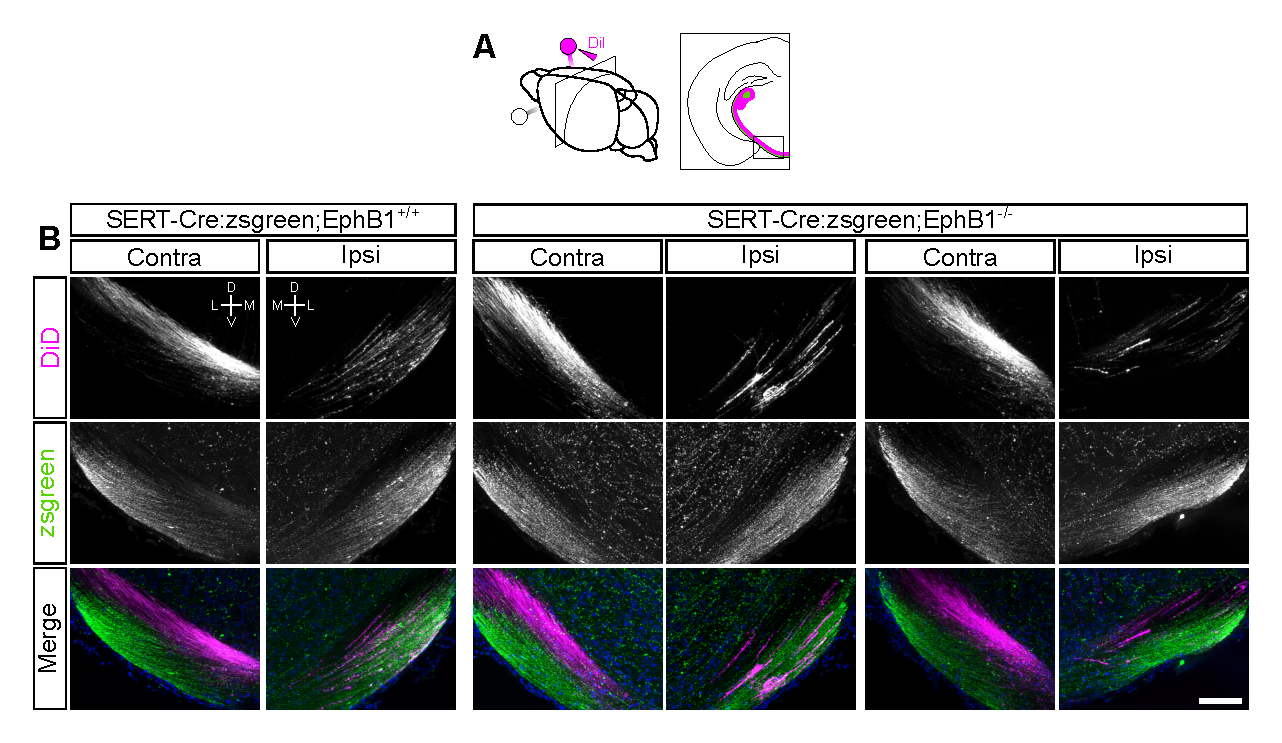
\includegraphics[width=\textwidth]{Figures/ESC_frontal_122_125_119.pdf}
        \caption[Ipsi and contra RGC axons in the SERT-Cre:zsgreen;EphB1 optic tract.]
        {Ipsi and contra RGC axons in the SERT-Cre:zsgreen;EphB1 optic tract.
        A) Labeling schema.
        DiD was placed onto the optic nerve head of P0 SERT-Cre:zsgreen;EphB1\textsuperscript{+/+} and SERT-Cre:zsgreen;EphB1\textsuperscript{-/-} fixed heads.
        Samples were sectioned 75$\mu$m thick in the frontal plane.
        B) DiD and zsgreen in the optic tract contra- and ipsilateral to the labeled retina.
        One control sample is shown (at left) and two EphB1\textsuperscript{-/-} samples (middle and right).
        Ipsi DiD axons are less well organized in the SERT-Cre:zsgreen;EphB1\textsuperscript{-/-} samples compared to control.
        Zsgreen label is similar across samples.
        Blue is Hoechst.
        D=dorsal, V=ventral, L=lateral, M=medial.
        Scale=100$\mu$m.}
        \label{ESCfrontal}
    \end{center}
\end{figure}

Figure~\ref{ESChorizontal} shows a second littermate pair, one SERT-Cre:zsgreen;EphB1\textsuperscript{+/+} and one SERT-Cre:zsgreen;EphB1\textsuperscript{-/-}, sectioned in the horizontal plane.
Again in these samples, the discombobulation of the remaining ipsi fibers is apparent in the mutant optic tract.
Both genotypes have a few stray fibers in the more medial aspect of the tract in these particular samples.
Medial fibers like these are sometimes visible in horizontal sections of wild-type animals in sections nearest the optic chiasm, and may represent axons that project to accessory visual targets.
However, comparing the DiD\textsuperscript{+} axons in just the more lateral aspect of the tract, the remaining fibers in the SERT-Cre:zsgreen;EphB1\textsuperscript{-/-} tract appear less well organized than those in the control SERT-Cre:zsgreen;EphB1\textsuperscript{+/+} tract.
As in the samples shown in the frontal plane, the zsgreen\textsuperscript{+} region looks comparable between genotypes, with no obviously straying zsgreen\textsuperscript{+} axons in the medial optic tract.
\begin{figure}[hbtp]
    \begin{center}
        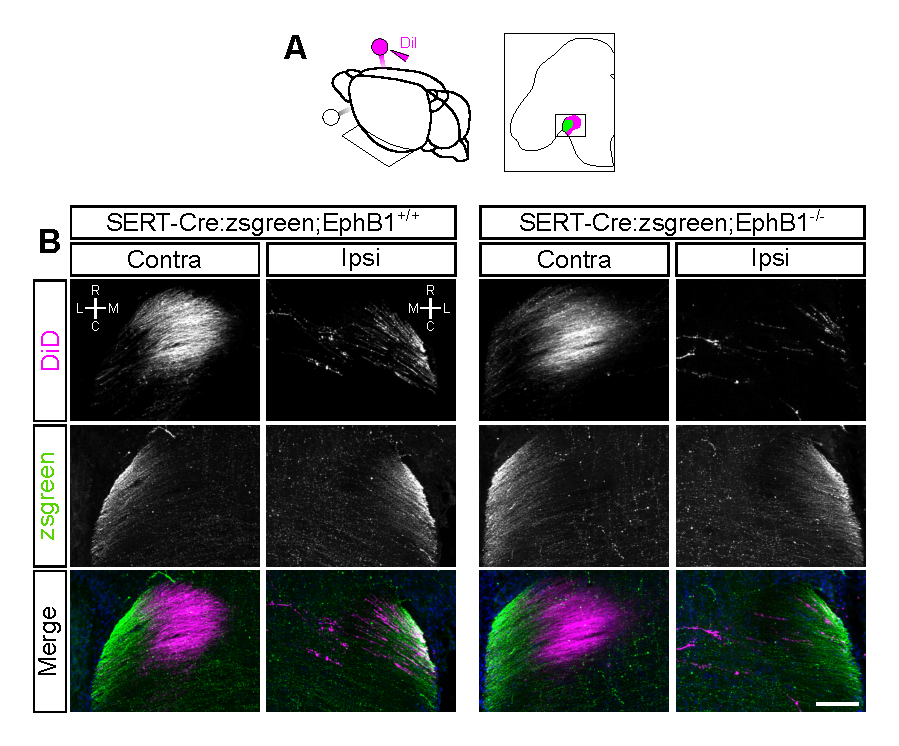
\includegraphics[width=\textwidth]{Figures/ESC_horizontal_137_142.pdf}
        \caption[Ipsi and contra RGC axons in the SERT-Cre:zsgreen;EphB1 optic tract, in the horizontal plane.]
        {Ipsi and contra RGC axons in the SERT-Cre:zsgreen;EphB1 optic tract, in the horizontal plane.
        A) Labeling schema.
        DiD was placed onto the optic nerve head of P0 SERT-Cre:zsgreen;EphB1\textsuperscript{+/+} and SERT-Cre:zsgreen;EphB1\textsuperscript{-/-} fixed heads.
        Samples were sectioned 75$\mu$m thick in the horizontal plane.
        B) DiD and zsgreen in the optic tract contra- and ipsilateral to the labeled retina.
        Ipsi DiD axons are more sparse and less well organized in the SERT-Cre:zsgreen;EphB1\textsuperscript{-/-} samples compared to control.
        Zsgreen label, however, is similar across samples.
        Blue is Hoechst.
        D=dorsal, V=ventral, R=rostral, C=caudal.
        Scale=100$\mu$m.}
        \label{ESChorizontal}
    \end{center}
\end{figure}

Finally, Figure~\ref{ESCVTfrontal} shows SERT-Cre:zsgreen;EphB1\textsuperscript{+/+} and SERT-Cre:zsgreen;EphB1\textsuperscript{-/-} samples labeled with DiD only in the VT region of the right retina.
Selectively labeling the VT retina with DiD should make it easier to compare the organization of VT contra axons between genotypes.
In SERT-Cre:zsgreen;EphB1\textsuperscript{-/-} samples, VT contra axons are a combination of ``true'' contra axons and misrouted axons (which should express \emph{SERT}).
Initial findings from this labeling schema confirm the findings from the previous two figures: contra DiD\textsuperscript{+} axons invade the zsgreen\textsuperscript{+} lateral optic tract in the SERT-Cre:zsgreen;EphB1\textsuperscript{-/-} sample, indicating that misrouted axons from the VT retina associate with the remaining ipsi axons from the other side.
Focal VT anterograde tracing is inherently more variable than whole eye anterograde, so this assessment needs additional cases before drawing definitive conclusions.
Additionally, confocal microscopy will be necessary to definitively assess colocalization of DiD and zsgreen labels in individual axons. 
\begin{figure}[hbtp]
    \begin{center}
        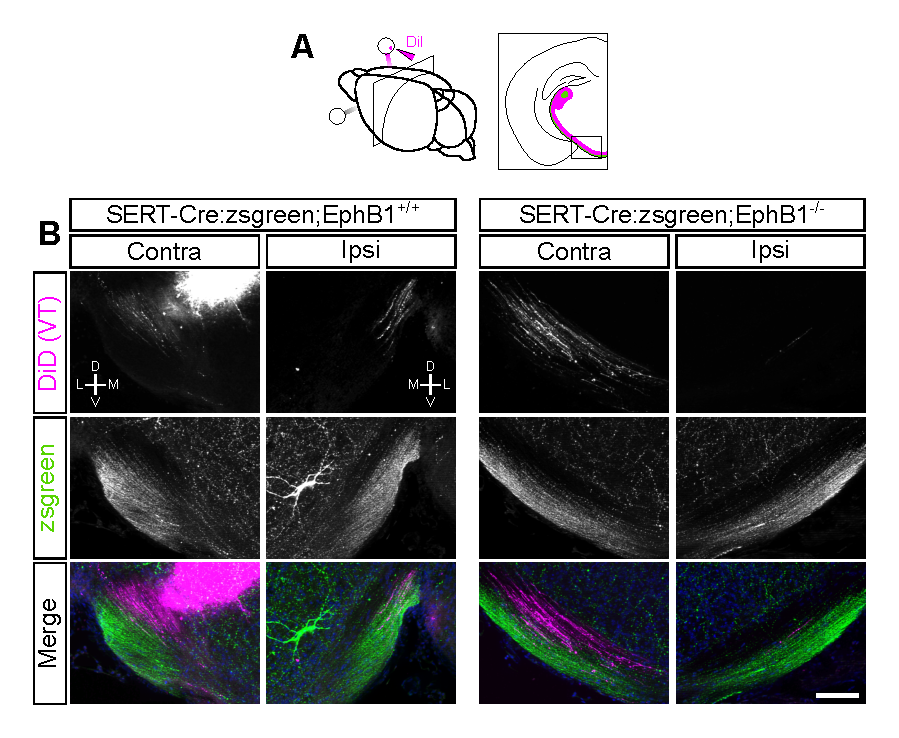
\includegraphics[width=\textwidth]{Figures/ESC_VT_frontal.pdf}
        \caption[RGC axon segregation in the SERT-Cre:zsgreen;EphB1 optic tract with focal anterograde tracing.]
        {RGC axon segregation in the SERT-Cre:zsgreen;EphB1 optic tract with focal anterograde tracing.
        A) Labeling schema.
        DiD was placed into the ventrotemporal (VT) retina of P0 SERT-Cre:zsgreen;EphB1\textsuperscript{+/+} and SERT-Cre:zsgreen;EphB1\textsuperscript{-/-} fixed heads.
        Samples were sectioned 75$\mu$m thick in the frontal plane.
        B) DiD and zsgreen were imaged in the optic tract contra- and ipsilateral to the labeled retina.
        Note that the zsgreen\textsuperscript{+} cell in the SERT-Cre:zsgreen;EphB1\textsuperscript{+/+} ipsi sample is outside of the optic tract and unrelated.
        Additionally, there is DiD artifact labeling in the brain on the contra side of the sample.
        D=dorsal, V=ventral, L=lateral, M=medial.
        Scale=100$\mu$m.}
        \label{ESCVTfrontal}
    \end{center}
\end{figure}